We present the experimental results of \sys performance. We start with describing the hardware environment (Section~\ref{sec:results_hardware}) followed by the software environment (Section~\ref{sec:results_software}) and we concluded by the evaluation results (Section~\ref{sec:results_evaluation}).

\subsection{Hardware Suite Description}
\label{sec:results_hardware}

In all experiments we used the following computing hardware: WISP\,5.1~\cite{wisp5,wisp}, i.e. build around MSP430FR5969~\cite{wolverine} 64\,kB FRAM microcontroller, and TI's MSP430FR5969 launchpad~\cite{MSP-EXP430FR5969_launchpad} (hardware type will be specified per experiment in Section~\ref{sec:results_evaluation}). WISP\,5.1 has been re-programmed during experiments using TI's Flash Emulation Tool (FET)~\cite{fet} with TI Code Composer Studio version X~\cite{}\todo{Report on CCS version}{Amjad}. FET was also used as a power supply in non-intermittent power experiment. To measure energy consumption of all benchmark applications (please refer to Section~\ref{sec:results_software}) Carnegie Mellon's EDB~\cite{edb} was used. In experiments involving wireless power, WISP was powered through an RFID reader (Impinj R1000 with firmware version 3.2.4.240~\cite{r1000_data_sheet}) connected to Liard RFMAX S9028PCRJ 8\,dBic~\cite{atlas2015}. RFID reader is controlled by a PC running Ubuntu 10.4 executing open source Python-based \emph{sllurp} library~\cite{sllrp_github} enabling low-level RFID reader control. Transmitted power of the RFID reader was 30\,dBm at 915\,MHz center frequency. For distance controlled experiments, WISP was positioned at varying length hollow paper tubes placed directly on a flat lying antenna. Code completion measurements have been performed using Salea~\cite{saleae} digital logic analyzer.

We also had alternative setup where we used MSP-TS430RGZ48C launchpad for continuous power experiment. We used internal timer for measuring run time. For harvested energy, we used ThingMagic Astra-EX RFID reader with power level of 17.25-30dBm. We used EDB~\cite{edb} for run time measurement. Applications were cross compiled using GCC and Clang, so that we can use LLVM for \sys compiler.

\subsection{Software Suite Description}
\label{sec:results_software}

We compare \sys against state of the art intermittent execution approach---Chain~\cite{chain}. We are not comparing \sys against DINO~\cite{dino} or Mementos~\cite{mementos} (Refer to Section~\ref{sec:background_consistency}), as (i) Chain is the only modular execution model available to which we can compare \sys, and (ii) Chain proves already its superiority over sequential model counterparts (i.e. DINO and Mementos).

We need to note that although another very relevant task-based runtime has been recently presented and referenced many times throughout this paper---Alpaca~\cite{alpaca} (written by the same group as Chain)---except the recently accepted manuscript we did not have the access to Alpaca's code during the preparation of this paper. Therefore Alpaca was excluded from the evaluation. \todo{Check if the line of argument is solid for the above paragraphs about not selecting DINO, Memenos and Aplaca}{Brandon}

The applications that were used in the evaluation are: (i) \textbf{Bitcount}: counts bits in x y byte pseudo-random string using x algorithms. Each result is compared for correctness; (ii) \textbf{Cold chain}: emulates embedded temperature sensing engine: measurements are randomly generated and are compressed using LZW algorithm for x-entry dictionary and y-byte block; (iii) \textbf{Cuckoo}: implements cuckoo filter---x entry filter filled to y of capacity---program first stores a sequence of pseudo-random numbers, then queries the filter to recover it; (iv) \textbf{RSA}: encrypts predefined x byte long string with a y bytes long key\todo{were keys of 64 bytes tested? If yes: d they exhaust energy}{Amjad}. This set of benchmarks is the same as used in~\cite{chain,alpaca}\todo{Fill-in the missing data and verify its correctness}{Przemek/Amjad}. In addition to Chain benchmarks new applications were implemented: (v) \textbf{DFT}, (vi) \textbf{Huffman compressor}, and (vii) \textbf{Selection Sort}. All applications are compared in Table~\ref{table:benchmark_list} in terms of source lines of code against Chain. \todo{finalize describing all applications once all experiments are done}{Przemek}

\begin{table}[t]
	\centering
	\footnotesize
	\begin{tabular}{|c|c|c|}
		\hline
		Nickname & SLOC (\sys) & SLOC (Chain~\cite{chain})\\
		\hline\hline
		Bitcount & 351 & 588 \\ %59\%
		Cold chain & 388 & 721 \\ %53\%
		Cuckoo & 483 & 762 \\ %63\%
		RSA & 887 & 1233 \\ %71\%
		DFT & {} & {} \\ %Two resolutions: 4 and 8 Bytes
		Huffman & {} & {} \\ %Data decompression size: 100 bytes
		Selection sort & {} & {} \\
		\hline
	\end{tabular}
\caption{List of benchmark programs used in \sys evaluation; SLOC: source lines of code.}
\label{table:benchmark_list}
\end{table}

\subsection{Evaluation Results}
\label{sec:results_evaluation}

\subsubsection{Compiler Performance}
\label{sec:results_compiler}

\begin{table}[t]
	\centering
	\footnotesize
	\begin{tabular}{|c|c|c|c|c|c|c|c|}
		\hline
		{} & \multicolumn{2}{l|}{{PVAR size (Byte)}} & \multicolumn{2}{c|}{{No. tasks}} & \multicolumn{2}{c|}{{No. paging code}} \\
		\hline
		Nickname & Hand & Comp. & Hand & Comp. & Hand & Comp. \\
		\hline\hline
		Bitcount & 22 & 22 & 10 & 15 & 81 & 93 \\
		Cold chain & 3492 & 3242 & 12 & 9 & 92 & 123 \\
		Cuckoo & 282 & 288 & 15 & 6 & 90 & 76 \\
		RSA & 332 & 250 & 20 & 27 & 130 & 296 \\
		AR & 166 & 218 & 11 & 6 & 112 & 333 \\
		Sort & 104 & 104 & 4 & 2 & 70 & 23 \\
		\hline
	\end{tabular}
	\caption{Comparison between compiler-generated \sys code (Comp.) and hand-written \sys code (Hand).}
\label{table:compiler_result}
\end{table}

We start with evaluating the efficiency of a \sys compiler. Table~\ref{table:compiler_result} shows the difference in the number of protected variables (PVAR), number of tasks, and number of inserted paging calls in the code between (i) hand-written \sys and (ii) compiler-generated \sys code. On average, compiler-generated code is only worse by 0.3\% in the number of protected variables. Regarding the number of tasks, compiler-generated code is better by roughly 16\%. The result indicate that \sys compiler is selecting boundaries better than the programmer doing it manually. However, \sys compiler should insert paging code conservatively when it {\em may} access protected variables, due to limitation of pointer alias. Thus, it results in \sys compiler introducing 48\% more paging code than programmer-written code (the results on run time for various \sys code versions is provide in Section~\ref{}). The performance is worse than programmer-written \sys code in overall, meaning the programmer should structure the code manually if the performance is critical; otherwise compiler can be used to simplify the programmability. 

Additionally, we evaluated the compile time for automatic task generation per application\footnote{We could not compile DFT application since it was using built-ins for C math functions (i.e. \texttt{rand()}, \texttt{sinf()}, \texttt{cosf()}) that were not provided by the Clang MSP430 back-end.}. The result are given in Table~\ref{table:compile_time}. Most of the compile time was due to pointer aliasing.\todo{Comment on: whether these times are good or bad; why there is such a difference in time between all applications; how many runs you performed; what PC/OS you used to run the code; how the result was measured; why results are rounded (there are no decimals in your result); what is "Clang MSP430 back-end"}{Kiwan}

\begin{table}[t]
	\centering
	\footnotesize
	\begin{tabular}{|c|c|c|c|c|c|}
		\hline
		Bitcount & Cold chain & Cuckoo & RSA & AR & Sort \\
		\hline\hline
		3 & 2 & 6 & 86 & 34 & > 1 \\
		\hline
	\end{tabular}
	\caption{\sys compile time per application (seconds).\todo{for Sort:">" or "<"?}{Kiwan}}
\label{table:compile_time}
\end{table}

\subsubsection{Task Coalescing Performance}
\label{sec:results_coalescing}

\begin{figure}
	\centering
	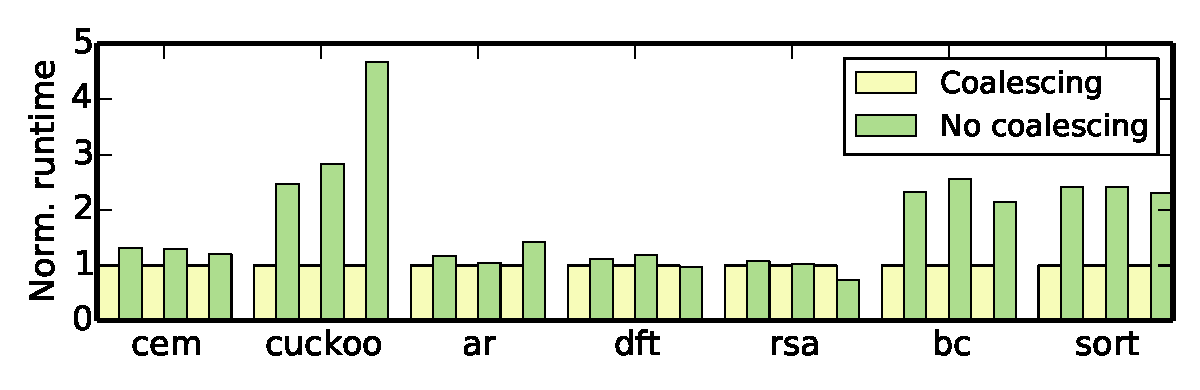
\includegraphics[width=\columnwidth]{figures/coalescing}
	\caption{Performance of \sys's  tasks coalescing mechanism compared to virtual task size equal to one (per application) at multiple WISP to RFID reader antenna distances.\todo{Replace "coal" with "coalescing", "No-coal" with "No coalescing"; use markers in addition to color; decide on uniform naming for apps (either all small or capitalized)}{Amjad}}
	\label{fig:coalescing}
\end{figure}

Experimental evaluation of task coalescing mechanism under intermittent power of \sys is given in Figure~\ref{fig:coalescing}. For each application we measured execution time (with and without task coalescing) at \{20, 40, 60\}\,cm distance between RFID antenna and WISP and when WISP was powered directly from FET. Each measurement was repeated x times per each distance/application. From the result we clearly see an enormous benefit of coalescing, especially at large WISP to RFID reader antenna distance ($\approx$56\% for cem, 100\% for sort and $\approx$400\% for bc). At each distance, \sys coalescing mechanism provided faster execution times compared to non-coalescing case. \todo{Discuss different shapes per app}{Amjad}

\begin{figure}
	\centering
	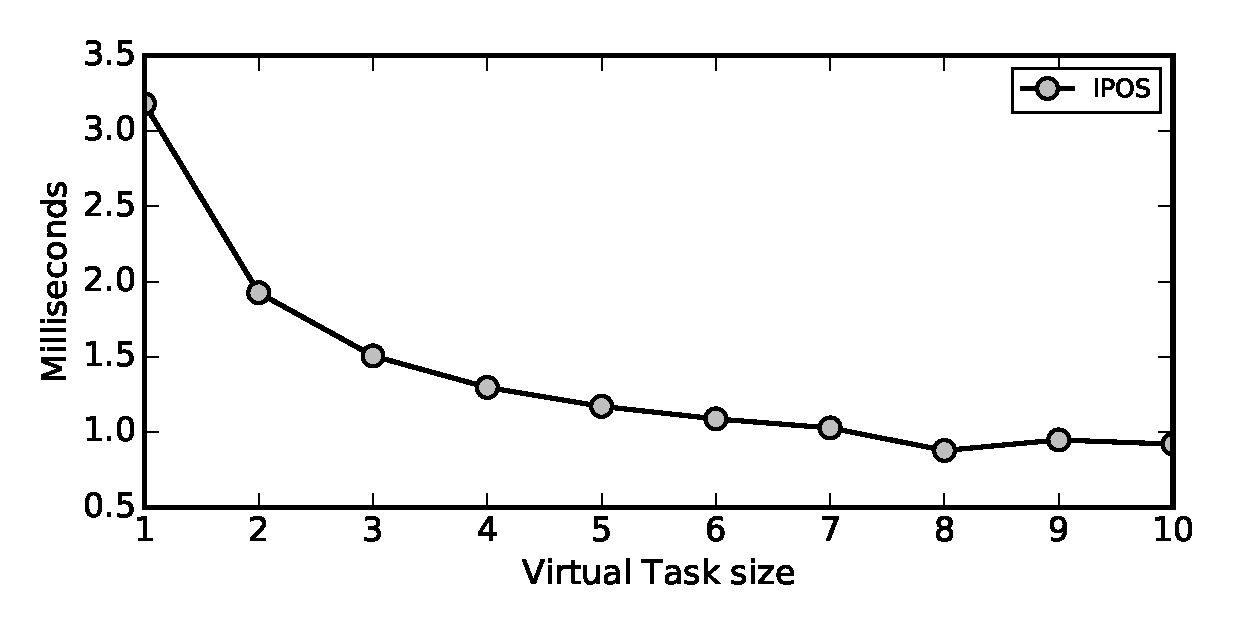
\includegraphics[width=\columnwidth]{figures/virtualTaskSize.eps}
	\caption{Execution time of a dummy application containing twelve empty tasks as a function of coalescing factor. We observe three times improvement from coalescing until four virtual tasks, while we observe a diminishing return from task coalescing beyond four. \todo{Improve the figure: make it narrower, larger font, remove legend, do not capitalize "Task" in X axis, add Y axis label (Execution time (ms))}{Amjad}}
	\label{fig:virtualTaskSize}
\end{figure}

The question remains: does coalescing all program's tasks into a singe virtual task (as the energy becomes fully available, i.e. from energy harvesting to continuous power environment) is the best one?. To answer this question we have implemented a simple program composed of $x$ empty tasks. We execute the same program by increasing coalescing factor by one while the device on which the program was executed was running on a stable power supply (refer to Section~\ref{sec:methodology_evaluation} for details). The result is presented in Figure~\ref{fig:virtualTaskSize}. We observe a significant increase in execution time as task are coalescent from one to four (three times execution time improvement). However, as the coalescing increases beyond four, we observe diminishing returns from coalescing in terms of execution time. \todo{Decide whether to place this figure in Evaluation section or leave it here}{Przemek}

\begin{figure}
	\centering
	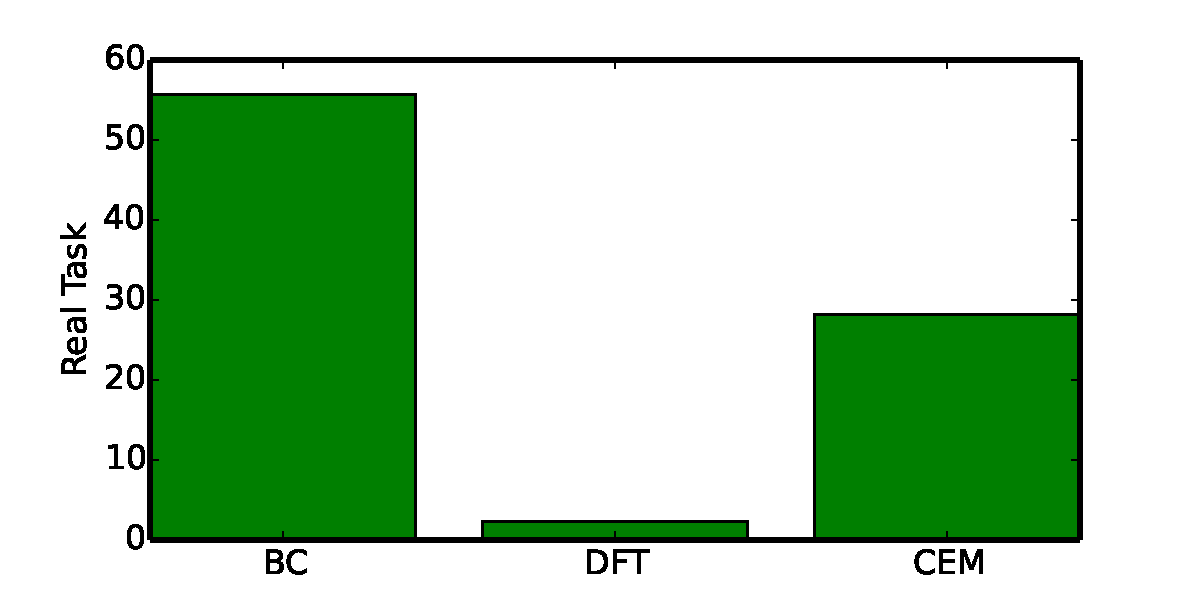
\includegraphics[width=\columnwidth]{figures/averageVirtualTaskSize}
	\caption{Average virtual task size (measured in real task unit\todo{Define real task unit}{Amjad}) of the virtual task sizes that the coalescing algorithm used to accomplished the applications at a WISP to RFID reader distance of 60\,cm.\todo{Please rewrite this sentence}{Amjad}}
	\label{fig:aveVirtuTaskSize}
\end{figure}

Measured size of tasks for each application is given in Figure~\ref{fig:aveVirtuTaskSize}.

Expected results:
\begin{itemize}
	\item performance for each application comparing bars for Chain, no coalescing/hand-tasked, coalescing/hand-tasked, no-coalescing/compiler, coalescing/compiler. Performance depicted, normalized to one of the configurations (probably Chain). This plot will cover most of the eval dimensions that we care about.
	\item Sensitivity plot---show amount of task merged, time to completion, overhead (in terms of task-size/cap-size sweep (remember we can vary either with approximately the same effect)), energy consumed. All experiments for fixed power, at 3 distances with wireless power, compared against Chain for 3 task/cap size configurations
\end{itemize} 

%Point for decision after main figure is ready

%Pull the compiler stuff into its own plot that compares compiler to hand-tasked, maybe only for the coalescing fig.  This reduces bars in plot 1, but runs the risk of making the compiler sound secondary, which we do not want to do.

%*Report only Chain, coalescing/hand-tasked, coalescing/compiler in the main plot.  This says that coalescing is the "default configuration" for VIPER. Later, in a second figure, we compare coalescing to no coalescing for hand-tasked and compiler as a characterization plot.

\todo{Provide results and text to this section}{Amjad}

\subsubsection{Memory Management Performance}
\label{sec:results_memory_management}

\begin{figure}
	\centering
	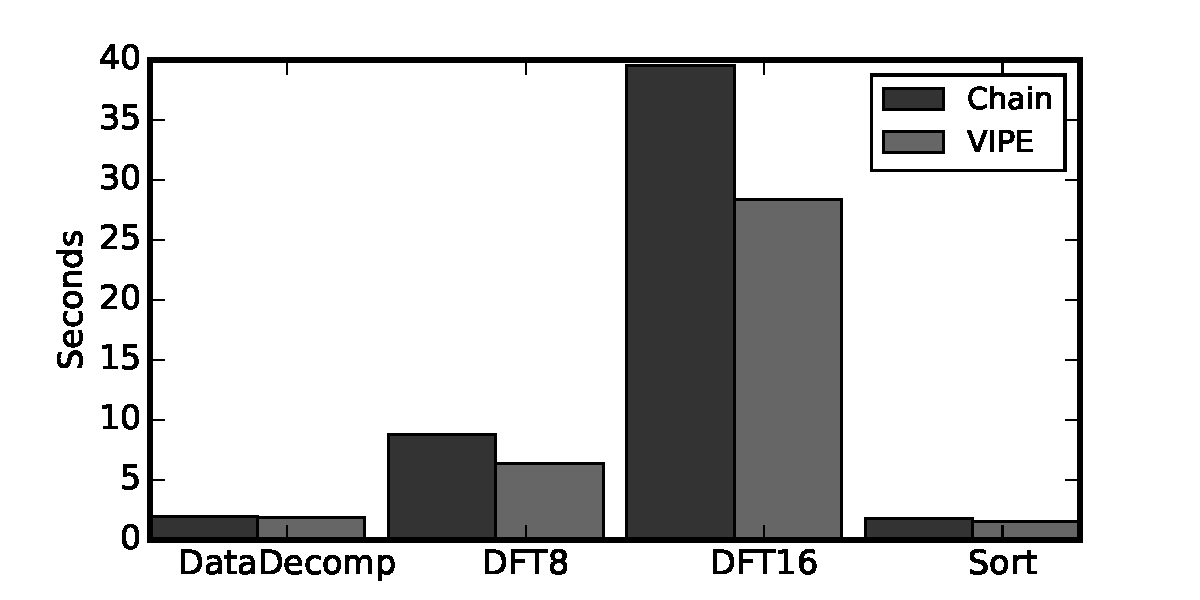
\includegraphics[width=\columnwidth]{figures/chain_vipe}
	\caption{Time to complete for a set of testing applications (refer to Table~\ref{table:benchmark_list}) using \sys versus Chain (no coalescing applied, fixed power supply). \todo{Figure placeholder---will be replaced with final one}{Amjad}}
	\label{fig:IPOSPerformance}
\end{figure}

\begin{figure}
	\centering
	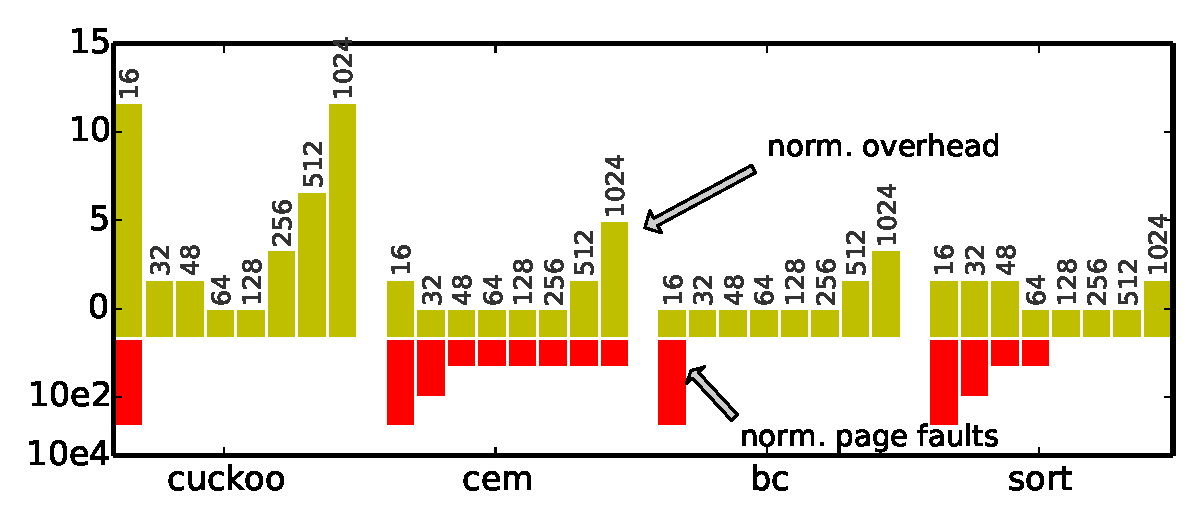
\includegraphics[width=\columnwidth]{figures/pagSizeOverhead}
	\caption{Normalized page size overhead and page faults per benchmark.\todo{Figure placeholder---will be replaced with final one}{Amjad}}
	\label{fig:IPOSPerformance}
	\label{fig:page_size}
\end{figure}

Figure~\ref{fig:page_size} presents the result on the effect of page swap size on the execution time of the programs executed by \sys. Overhead has been measured in the MCU clock cycles with values provided by TI CCS. Result has been normalized per benchmark: for the overhead results---to the minimum obtained value and for page faults---to the third measured maximum value\todo{Check again}{Amjad}. A subset of applications has been selected for evaluation. Additionally, page faults have been measured. The result show clearly a bathtub-shape bar plot for each application, demonstrating that for each application there is always a page size that minimizes \emph{both} execution time and page swaps. For all applications (except for Sort) this value equals roughly to 64 bytes. The shape of each figure can be explained as follows. For small page sizes (<64) the execution time is dominated by the \emph{frequency} of page swaps (each swap takes non-zero time, as shown in Figure~\ref{fig:dmaTimeEnergy}). On the other hand, in the opposite case the execution time is dominated by the time of swapping of one large page from SRAM to FRAM. Another interesting observation is the non-symmetric shape of each bar plot. This is due the size of data manipulated by the program: minimum point of overhead equals roughly to the size of the variables manipulated by each benchmark. Worth noting is also large discrepancy between minimum and maximum overhead for each benchmark (e.g. for Cuckoo 8 (at 16 bytes) to 1 (at 64 bytes), BC: 1 (at 16 bytes) to $\approx$2 (at 1024 bytes)). \todo{Explain this phenomenon}{Amjad}

\subsubsection{Case Study}
\label{sec:case_study}

The final experiment assessing usefulness of \sys's use in real application. For this we have a implemented an battery-less wirelessly-powered sound detector as an example. To the best of our knowledge, this is the first case study that demonstrates a intermittently-powered system supplied by harvested energy at runtime, which continuously interacts with real-life signals. 

The application aims at detecting a specific tone in the audio signal (in the implementation: 1\,kHz) based on on-the-fly audio measurement. For this we have connected an analog MEMS microphone~\cite{microphone} output to AUX3 port of WISP\,5.1 (while the microphone was powered directly by WISP, which was then wirelessly power-supplied by the RFID reader). Audio signal is sampled by the microcontroller's ADC and passed to the FFT function (internal function of the TI's Digital Signal Processing library~\cite{ti_dsp}) to find a tone above a predefined threshold. The output of the detection is signalled by the WISP on-board LED. The video of demonstrating the working system is available via \url{https://link_to_a_video}.

Expected results:
\begin{itemize}
	\item Compare execution time: \sys against Chain for X\,s long audio signal detection at two antenna distances
	\item Make a video of the demonstration 
\end{itemize}
 
\todo{Check if we really need this application}{Brandon}
\todo{Provide results and text to this section---if time allows (this result is not critical)}{Amjad/Przemek}
